\thispagestyle{empty}

\mbox{ }

\vfill

\begin{center}
  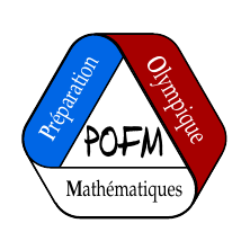
\includegraphics[width=4cm]{01-Intro/logos/pofm.png}

  \vspace{1cm}

  Retrouvez le polycopié avec l'ensemble des cours et exercices du stage\\
  ainsi que toutes les informations au sujet de la POFM\\
  sur notre site internet

  \smallskip

  \textbf{\texttt{https://maths-olympiques.fr}}

  \bigskip

Voici également quelques liens utiles pour poursuivre le travail réalisé pendant ce stage :
%\refstepcounter{dummy}
% \label {liensutiles}
\begin{itemize}
\item le site d'Animath : \href{http://www.animath.fr}{animath.fr} ;
\item le site de la POFM : \href {http://www.maths-olympiques.fr}{maths-olympiques.fr} et notamment
\item les archives de problèmes (polycopiés etc\ldots) : \href{http://www.maths-olympiques.fr/?page_id=41}{maths-olympiques.fr/?page\_id=41} ;
\item le site \emph{Mathlinks} : \href{http://www.mathlinks.ro}{mathlinks.ro} ;
\item le site \emph{Art of Problem Solving} : \href{https://www.artofproblemsolving.com}{artofproblemsolving.com}.
\end{itemize}

\end{center}

\vfill